\documentclass[11pt,aspectratio=169]{beamer}

% -------------------- THEME & LAYOUT --------------------
\usetheme{Madrid}
\usecolortheme{dolphin} % base color scheme
\usefonttheme{professionalfonts}
\setbeamercovered{transparent}
\setbeamertemplate{navigation symbols}{}   % remove navigation buttons
\setbeamertemplate{caption}[numbered]      % numbered captions
\setbeamertemplate{itemize items}[triangle]
\setbeamersize{text margin left=1.2cm,text margin right=1.2cm} % adjust to taste

% -------------------- GLOBAL FONT SETTINGS --------------------

% 1. Force the base beamer font to small
\setbeamerfont{normal text}{size=\small}

% 2. Force math environments to follow the "small" font size
\setbeamerfont{math text}{size=\small}
\setbeamerfont{equation}{size=\small}

% 3. Redefine \normalsize itself 
% This ensures equations and lists (which look for \normalsize) use  instead.
\let\oldnormalsize\normalsize
\renewcommand{\normalsize}{\oldnormalsize\small}

% 4. Ensure lists also stay small
\setbeamerfont{itemize/enumerate body}{size=\small}
\setbeamerfont{itemize/enumerate subbody}{size=\small}

% -------------------- FONTS & TYPOGRAPHY --------------------
\usepackage[T1]{fontenc}
\usepackage[utf8]{inputenc}
\usepackage{newpxtext,newpxmath} % Palatino-like font & math
\usepackage{microtype}

% -------------------- MATH, TABLES & GRAPHICS --------------------
\usepackage{amsmath,amssymb,amsfonts,mathtools}
\usepackage{bm,booktabs,siunitx,graphicx}
\graphicspath{{./}{./figures/}}

% -------------------- UTILITIES --------------------
\usepackage{appendixnumberbeamer}
\usepackage{ragged2e}
\usepackage{xspace}
\usepackage{csquotes}
\usepackage{xcolor}

% -------------------- HYPERREF --------------------
\hypersetup{
  colorlinks=false,
  pdfauthor={Francesca},
  pdftitle={Chapter 1 — The Value of Currency}
}

% -------------------- COLORS & EMPHASIS --------------------
\definecolor{myblue}{RGB}{0,70,140}
\definecolor{myred}{RGB}{180,30,30}
\definecolor{mygreen}{RGB}{0,120,70}
\definecolor{gold}{RGB}{184,134,11}

\setbeamercolor{title}{fg=gold}       % title page
\setbeamercolor{frametitle}{fg=gold}  % slide titles
\setbeamercolor{structure}{fg=gold}   % bullets, sections, links
\setbeamercolor{section in head/foot}{fg=gold,bg=black!10} % gold text on light background

% -------------------- FOOTLINE --------------------
\setbeamertemplate{footline}{
  \leavevmode%
  \hbox{%
    % Section links (hidden if no current section)
    \begin{beamercolorbox}[wd=0.7\paperwidth,ht=2.5ex,dp=1.5ex,leftskip=1.4em]{section in head/foot}%
      \ifx\insertsection\empty
        % nothing
      \else
        Section: \insertsection
      \fi
    \end{beamercolorbox}%
    % Frame number right
    \begin{beamercolorbox}[wd=0.3\paperwidth,ht=2.5ex,dp=1.5ex,leftskip=3.8cm]{section in head/foot}%
      \insertframenumber/\inserttotalframenumber
    \end{beamercolorbox}%
  }%
  \vskip1pt%
}



\newcommand{\highlight}[1]{\textcolor{myblue}{#1}}
\newcommand{\warning}[1]{\textcolor{myred}{#1}}

% -------------------- SHORTCUTS --------------------
\newcommand{\E}{\mathbb{E}}
\newcommand{\R}{\mathbb{R}}
\newcommand{\dd}{\mathrm{d}}
\newcommand{\mc}[1]{\mathcal{#1}}
\newcommand{\bb}[1]{\mathbb{#1}}
\newcommand{\uc}{U_c}
\newcommand{\zg}{Z_g}

% -------------------- TIGHTER DISPLAY MATH --------------------
\makeatletter
\g@addto@macro\normalsize{%
  \setlength\abovedisplayskip{8pt}%
  \setlength\belowdisplayskip{8pt}%
  \setlength\abovedisplayshortskip{6pt}%
  \setlength\belowdisplayshortskip{6pt}%
}
\makeatother
\setbeamertemplate{frametitle}{
  \nointerlineskip
  \begin{beamercolorbox}[wd=\paperwidth,ht=3.5ex,dp=1ex,center]{frametitle}
    \centering\insertframetitle
  \end{beamercolorbox}
}

% -------------------- Bibliography --------------------
\usepackage[backend=biber,style=authoryear]{biblatex}
\addbibresource{sources.bib}


% -------------------- METADATA --------------------
\title[Part I — Currency and Money]{\textbf{Part I: Currency and Money}\\[2pt]\large Chapter 2 — Cash as a Medium of Exchange}
\author{Severin Rothen}
\institute{}
\date{\today}

% -------------------- SECTION ROADMAP --------------------
\AtBeginSection[]
{
  \begin{frame}
    \tableofcontents[currentsection, hideothersubsections]
  \end{frame}
}


\begin{document}

%- ===================== TITLE SLIDE =====================
\begin{frame}[plain] % 'plain' removes header/footer for the title slide

\begin{columns}[T,totalwidth=\textwidth]

% ----- Left column: Main title, professor, chapter -----
\begin{column}{0.45\textwidth}
\vspace{2cm}

% Main title
{\usebeamercolor[fg]{title}\LARGE\textbf{Monetary Economics}\\[0.3cm]
\LARGE\textbf{and Policy}} 

\vspace{0.5cm}

% Professor name and date
{\large\textit{Pierpaolo Benigno}}\\[0.1cm]

\vspace{1cm}

% Chapter and subtitle
{\usebeamercolor[fg]{frametitle}\large Chapter 2: Cash as a Medium of Exchange}

\end{column}

% ----- Right column: Image -----
\begin{column}{0.55\textwidth}
\vspace{1cm}
\centering
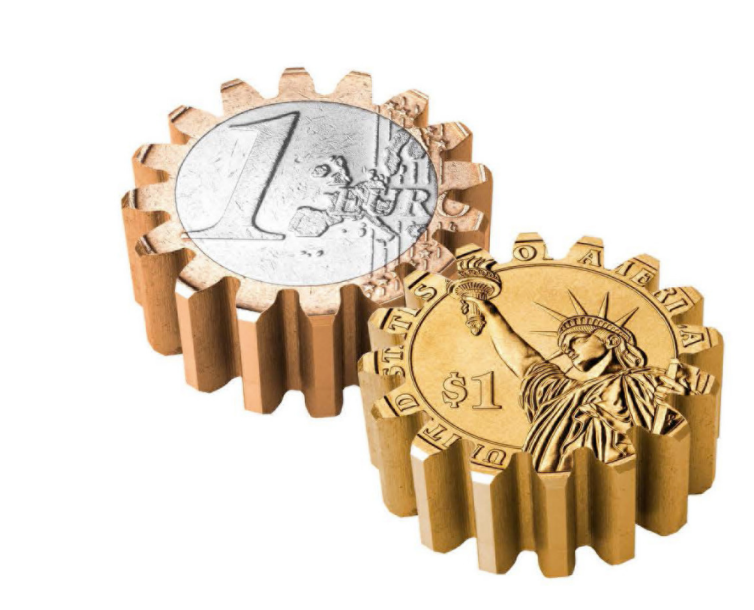
\includegraphics[width=0.9\linewidth]{Cover.png}
\end{column}

\end{columns}

% ----- Footer text (bottom-right corner) -----
\vspace*{2cm} % adjust if needed
\hfill{\large\textit{Prepared by Severin Rothen}}

\end{frame}

\begin{frame}{What We Will Learn}
\small
\begin{itemize}

    \item Why cash (banknotes and coins) is introduced explicitly as a \textbf{medium of exchange} and how this differs from Chapter~1.

    \vspace{0.6em}

    \item How this affects money demand and price determination.

    \vspace{0.6em}


    \item Price-level determination under:
    \begin{itemize}
        \item an interest-rate rule (FTPL and CBTPL),
        \item control of monetary aggregates,
        \item the \textbf{Gold Standard},
        \item \textbf{cryptocurrency competition}.
    \end{itemize}

    \vspace{0.6em}

    \item What stablecoins are.

\end{itemize}
\end{frame}


% OUTLINE
\begin{frame}{Outline}
\tableofcontents
\end{frame}

% Equation numbering
\setcounter{equation}{0}
\renewcommand{\theequation}{2.\arabic{equation}}


% =====================================================
\section{Introduction}
% =====================================================
% Hume -> Smith -> Monetarism
% Monetary system with no backing as a discontinuity
\begin{frame}{Currency as a Medium of Exchange}
\small
\begin{itemize}

    \item This chapter introduces currency (cash and banknotes) explicitly as a \textbf{medium of exchange}.

    \vspace{0.6em}

    \item We will refer to currency as \textbf{money}, although money need not be currency (as discussed in Chapter~1).

    \vspace{0.6em}

    \item The understanding of money and its quantity has deep historical roots.

    \vspace{0.8em}

    \item \textbf{David \textcite{hume1752money}} theorized, in a metallic system, that:
    \begin{itemize}
        \item An increase in the quantity of money is equivalent to an increase in the supply of gold and silver in a nation.
        \item A higher money supply raises the domestic price level, reducing exports and increasing imports.  
              As gold and silver flow out of the country, prices re-equalize internationally, restoring balance.
    \end{itemize}

\end{itemize}
\end{frame}

\begin{frame}{Historical Perspective on Money}
\small
\begin{itemize}

    \item For most of history, money circulated in the form of \textbf{coins with precious metal content}, although primitive forms of money (e.g., wampum, tobacco) were used even into the colonial American period.

    \vspace{0.8em}

    \item A major medieval innovation was the ability to \textbf{economize on gold in transactions}, giving rise to instruments such as \textbf{bills of exchange}.

    \vspace{0.8em}

    \item Later, in Venice and Amsterdam, public banks issued \textbf{account money}—a form of non-physical money backed by metal reserves on their balance sheets and used as a means of payment.

    \vspace{0.8em}

    \item The \textbf{real bills doctrine}, developed by \textbf{Adam \textcite{smith1776wealth}}, argued that currency could be backed by \textbf{private short-term commercial claims} rather than only by gold—though the system as a whole still relied on metallic backing.
    
\end{itemize}
\end{frame}
\begin{frame}{Intrinsically Worthless Currency I}
\small
\begin{itemize}

    \item The emergence of an \textbf{intrinsically worthless paper-money system} represents a major discontinuity, even if historically it evolved gradually from fully backed to partially backed paper money.

    \vspace{0.7em}

    \item Under such a system, currency becomes a \textbf{self-referential claim}—a promise to be paid in units of itself, without intrinsic value or commodity backing.

    \vspace{0.7em}

    \item This contrasts sharply with earlier commodity-based systems in which money had intrinsic metallic value.

\end{itemize}
\end{frame}

\begin{frame}{Intrinsically Worthless Currency II}
\small
\begin{itemize}

    \item Besides central-bank-issued money, \textbf{private agents can also issue money} (e.g., bank deposits, stablecoins).

    \vspace{0.7em}

    \item Privately issued money typically represents a \textbf{claim on central bank money} or other high-quality liquid assets.

    \vspace{0.7em}

    \item Despite the absence of intrinsic value, money remains \textbf{essential in the payment system}, facilitating transactions and coordinating economic activity.
    
\end{itemize}
\end{frame}

\begin{frame}{Monetarism: Historical Context}
\small
\begin{itemize}

    \item The shift from commodity-backed to \textbf{intrinsically worthless fiat currency} paved the way for monetarism.

    \vspace{0.7em}

    \item Milton Friedman’s \textit{A Program for Monetary Stability} \textcite{friedman1960program} is widely viewed as the modern foundation of monetarist thought.

    \vspace{0.7em}

    \item After the collapse of the \textbf{Bretton Woods system} in the early 1970s, several central banks attempted to target money aggregates as the central focus of monetary policy.

    \vspace{0.7em}

    \item Canada, the United Kingdom, and the United States later abandoned strict monetary targeting due to instability in money–inflation relationships.
    
\end{itemize}
\end{frame}

\begin{frame}{Monetarism: Ideas and Legacy}
\small

\textbf{Milton \textcite{friedman1960program}:} \textit{A Program for Monetary Stability}

\vspace{0.6em}

\begin{itemize}

    \item Modern foundation of monetarism.

    \vspace{0.6em}

    \item Monetarism holds that the \textbf{quantity of money strongly influences economic activity and the price level}.

    \vspace{0.6em}

    \item Monetary policy should therefore aim to \textbf{control the growth rate of the money supply}.

    \vspace{0.6em}

    \item Germany implemented a successful policy of targeting monetary aggregates for more than two decades, influencing the ECB’s adoption of a monetary pillar in its strategy.

\end{itemize}
\end{frame}



% =====================================================
\section{Model}
% =====================================================

% -----------------------------
\begin{frame}{Model Overview}
\textbf{Economic Setting}
\begin{itemize}
  \item Infinite-horizon, closed economy with perfect foresight
  \item Single consumption good $C$ with constant endowment $Y$
\end{itemize}

\textbf{Agents}
\begin{itemize}
  \item Representative consumer
  \item Treasury
  \item Central Bank (CB)
\end{itemize}

\textbf{One Currency = CB's liabilities}
\begin{itemize}
  \item Cash $M_t$
  \item Reserves $X_t$
\end{itemize}
\end{frame}

\begin{frame}{Representative Consumer: Preferences}
\small

\textbf{Intertemporal Utility}
\begin{align}
\sum_{t=t_0}^\infty 
\beta^{t-t_0}
\left[
    U(C_t)
    +
    V\!\left(\frac{M_t}{P_t}\right)
\right].
\label{2.1}
\end{align}

\vspace{0.8em}

\begin{columns}[T,totalwidth=\textwidth]

% -------- LEFT COLUMN --------
\begin{column}{0.48\textwidth}
\textbf{Properties of $U(C_t)$}
\begin{itemize}
    \item $U(\cdot)$ concave and differentiable.
    \item Argument: consumption good $C_t$.
    \item $U_c(C_t) > 0$,
          \quad $U_{cc}(C_t) < 0$.
\end{itemize}
\end{column}

% -------- RIGHT COLUMN --------
\begin{column}{0.48\textwidth}
\textbf{Properties of $V(M_t/P_t)$}
\begin{itemize}
    \item $V(\cdot)$ concave and differentiable.
    \item Argument: real money balances $M_t/P_t$.
    \item Satiation point $\bar{m} > 0$:
    \[
        V_m\!\left(\frac{M_t}{P_t}\right)=0
        \quad \text{for }
        \frac{M_t}{P_t} \ge \bar{m}.
    \]
    \item $V_m(\cdot)$ is the derivative of $V(\cdot)$.
\end{itemize}
\end{column}

\end{columns}

\end{frame}


\begin{frame}[label=orig_budget]{Budget Constraint}
\small
\textbf{Budget Constraint at time $t$}
\begin{align}
\frac{B_t+X_t}{1+i_t}+M_t+P_t C_t + T_t = B_{t-1}+X_{t-1}+M_{t-1}+P_t Y, \label{2.2}
\end{align} 

\textbf{Where}
\begin{itemize}
  \item $B_t$: default-free one-period bond (unit face value), discounted at nominal rate $i_t$
  \item $X_t$: CB reserves, paying $i_t^X$
  \item $M_t$: cash (zero interest)
  \item $P_t$: price of consumption good
  \item $T_t$: lump-sum taxes (negative = transfers)
  \item $Y$: constant endowment of goods
\end{itemize}

\textbf{Portfolio constraints}
\begin{itemize}
  \item Bonds: $B_t$ can be held as asset $(>0)$ or issued as debt $(<0)$
  \item Cash and reserves: $M_t \ge 0$, $X_t \ge 0 \ \forall \ t \ge t_0$
\end{itemize}
\end{frame}

\begin{frame}{Borrowing Limit}
\begin{itemize}
    
\item The consumer faces the borrowing limit:
\begin{align}
-\frac{B_{t-1}}{P_t}\le \frac{M_{t-1}+X_{t-1}}{P_t}+\sum_{j=0}^\infty R_{t,t+j}\left(Y-\frac{T_{t+j}}{P_{t+j}}\right) < \infty, \label{2.3}
\end{align}
where discount factor $R_{t,t+j}$ has the same definition as in Chapter 1. \\ \vspace{1em}

\item The consumer chooses $\left\{  C_t, B_t, X_t, M_t \right\}_{t=t_0}^{\infty}$ with $C_t, X_t, M_t \ge 0$ to maximize intertemporal utility (\ref{2.1}) subject to budget constraint (\ref{2.2}) and the borrowing limit (\ref{2.3}) at each time $t\ge t_0$ given initial conditions $B_{t_0-1}, X_{t_0-1}, M_{t_0-1}$.

\end{itemize}
\end{frame}

\begin{frame}{Intertemporal Budget Constraint}

\begin{itemize}
    \item An equivalent representation of the consumer’s problem can be obtained by replacing equation~(\ref{2.3}) with the intertemporal budget constraint:
\begin{align}
\sum_{t=t_0}^\infty R_{t_0,t}\left(
    C_t
    + 
    \underbrace{\frac{i_t}{1+i_t}\frac{M_t}{P_t}}_{\footnotesize\text{cost of holding money}}
\right)
\le 
\frac{B_{t_0-1}+X_{t_0-1}+M_{t_0-1}}{P_{t_0}}
+ 
\sum_{t=t_0}^\infty R_{t_0,t}\left(
    Y-\frac{T_t}{P_t}
\right).
\label{2.4}
\end{align}

\item The present discounted value of consumption and the cost of holding money (the interest rate forgone on real money balances) must not exceed initial real wealth plus the present discounted value of net endowment.
\end{itemize}
\end{frame}
\begin{frame}{Asset Limit Condition}

\begin{itemize}
    \item A third, equivalent formulation of the consumer’s problem replaces constraint~(\ref{2.4}) with:
    \begin{align}
    \lim_{t \to \infty} 
    \left\{ 
    R_{t_0,t} 
    \left( 
    \frac{B_{t-1} + X_{t-1} + M_{t-1}}{P_t}
    \right) 
    \right\} 
    \ge 0.
   \label{2.5}
    \end{align}
\vspace{0.5em}
    \item This condition requires that the limit of the discounted value of the household’s asset holdings remains non-negative.
\end{itemize}

\end{frame}


\begin{frame}{Consumer Optimality Conditions}
\small
\begin{itemize}
 \item Define the Lagrange multiplier $\lambda_t$ associated with constraint~(\ref{2.2}). Then $\lambda_t = U_c(C_t)/P_t$, where $U_c(\cdot)$ denotes the first derivative of the utility function $U(\cdot)$. 
 \vspace{0.35em}

 \item The first-order condition (FOC) with respect to $X_t$ or $B_t$ is:
 \begin{align}
 \frac{U_c(C_t)}{P_t}=\beta (1+i_t)\frac{U_c(C_{t+1})}{P_{t+1}}. \label{2.6}
 \end{align}

 \vspace{0.35em}
 \item The FOC with respect to $M_t$ implies:
 \begin{align}
 \frac{U_c(C_t)}{P_t}=\frac{1}{P_t}V_m(\frac{M_t}{P_t})+\beta \frac{U_c(C_{t+1})}{P_{t+1}}. \label{2.7}
 \end{align}
 or, using equation~(\ref{2.6}):
 \begin{align}
 1=\frac{V_m(\frac{M_t}{P_t})}{U_c(C_t)}+\frac{1}{1+i_t}. \label{2.8}
 \end{align}
\end{itemize}

\end{frame}
\begin{frame}{Money Demand}

\begin{itemize}

    \item Using equation~(\ref{2.8}), we can express the demand for real money balances as:
    \begin{align*}
        \frac{M_t}{P_t} \ge 
        V_m^{-1}\!\left( 
            \frac{U_c(C_t)i_t}{1+i_t}
        \right)
        \equiv 
        L\!\left(
            \underset{(+)}{C_t},\,
            \underset{(-)}{i_t}
        \right).
    \end{align*}

    \item When $i_t > 0$, the above relationship holds with equality.  
    The demand for real money balances increases with consumption and decreases with the nominal interest rate.

    \item When $i_t = 0$, the marginal utility of real money balances $V_m(\cdot)$ is zero, implying that households may hold any arbitrary amount of real money balances above the satiation level.
    
\end{itemize}

\end{frame}

\begin{frame}{Consumer Optimality: IBC or Transversality Condition}

\begin{itemize}
\item In the optimal allocation the intertemporal budget constraint~(\ref{2.4}) holds with equality, which means that no resources are thrown away: 

\begin{align}
\sum_{t=t_0}^\infty R_{t_0,t}\left(C_t + \frac{i_t}{1+i_t}\frac{M_t}{P_t}\right)
= \frac{B_{t_0-1}+X_{t_0-1}+M_{t_0-1}}{P_{t_0}} + \sum_{t=t_0}^\infty R_{t_0,t}\left(Y-\frac{T_t}{P_t}\right). \label{2.9}
\end{align}

\item Alternatively, the transversality condition holds, i.e., \eqref{2.5} holds with equality: 
\begin{align}
\lim_{t \to \infty} \left\{ 
R_{t_0,t} \left( \frac{B_{t-1} + X_{t-1} + M_{t-1}}{P_t}\right) \right\} = 0. \label{2.10}
\end{align}
\end{itemize}

\end{frame}

\begin{frame}{Government}
\begin{itemize}

\item The central bank's flow budget constraint is represented by:
\begin{align}
    \frac{B_t^C - X_t^C}{1 + i_t} - M_t^C = B_{t-1}^C - X_{t-1}^C - M_{t-1}^C - T_{t}^C, \label{2.11}
\end{align}
where money $M^C$ and reserves $X^C$ are the central bank's liabilities and $B^C$ the central bank's holdings of short-term default-free assets issued by the private sector or the treasury. 
\item The treasury's flow budget constraint is: 
\begin{align}
    \frac{B_t^F}{1+i_t} = B_{t-1}^F - T_t - T_t^C. \label{2.12}
\end{align}
where $B^F$ is the treasury's debt, $T$ are lump-sum taxes and $T^C$ are the nominal remittances received from the central bank. 
\end{itemize}

\end{frame}

\begin{frame}{Market Clearing}
\begin{itemize}
    \item In equilibrium, the markets for debt, reserves and money clear: 
\begin{align}
    B_t^F &= B_t^C + B_t, \label{2.13} \\
    X_t^C &= X_t, \label{2.14} \\
    M_t^C &= M_t \label{2.15},    
\end{align}
for each $t \ge t_0$
\vspace{0.25cm}
\item Equilibrium in asset markets together with the flow budget constraints of consumers and the government implies goods market equilibrium, $C_t = Y$ for each $t \ge t_0$.
\end{itemize}
\end{frame}

% --- First Slide ---
\begin{frame}{Equilibrium Conditions}
\small
\begin{itemize}

    \item The \textbf{central bank’s budget constraint} is:
    \begin{align}
        \frac{B_t^C - X_t}{1 + i_t} - M_t 
        = B_{t-1}^C - X_{t-1} - M_{t-1} - T_{t}^C.
        \label{2.16}
    \end{align}

    \item The \textbf{treasury’s budget constraint} is:
    \begin{align}
        \frac{B_t^F}{1+i_t} 
        = B_{t-1}^F - T_t - T_t^C.
        \label{2.17}
    \end{align}

    \item The \textbf{bond market clearing condition} requires that:
    \begin{align}
        B_t^F = B_t^C + B_t.
        \label{2.18}
    \end{align}

    \item The \textbf{intertemporal constraint on taxes}, identical to equation~(1.12) in Chapter~1, is given by:
    \begin{align}
        \frac{B_{t_0-1}^F}{P_{t_0}} 
        = \sum_{t=t_0}^\infty \beta^{t-t_0} 
        \left( 
            \frac{T_t}{P_t} + \frac{T_t^C}{P_t} 
        \right).
        \label{2.19}
    \end{align}

\end{itemize}
\end{frame}


% --- Second Slide ---
\begin{frame}{Equilibrium Conditions}
\small
\begin{itemize}

    \item The \textbf{Fisher equation} (from the first-order condition~(\ref{2.6}) and goods market clearing) links the nominal interest rate to expected inflation:
    \begin{align}
        1+i_t = \frac{1}{\beta}\frac{P_{t+1}}{P_t}.
        \label{2.20}
    \end{align}

    \item The \textbf{money market equilibrium condition} (from the money demand equation) is:
    \begin{align}
        \frac{M_t}{P_t} \ge L(Y_t, i_t),
        \label{2.21}
    \end{align}
    which holds with equality when $i_t > 0$.

    \item The \textbf{intertemporal resource constraint} (from combining equations~(\ref{2.9}) and~(\ref{2.4})) ensures that the present value of real government resources equals the initial real value of its liabilities:
    \begin{align}
        \sum_{t=t_0}^\infty \beta^{t-t_0}
        \left(
            \frac{T_t}{P_t} + \frac{i_t}{1+i_t}\frac{M_t}{P_t}
        \right)
        = 
        \frac{B_{t_0-1}+X_{t_0-1}+M_{t_0-1}}{P_{t_0}}.
        \label{2.22}
    \end{align}

\end{itemize}
\end{frame}

\begin{frame}{Equilibrium}
\small
An equilibrium is a set of sequences $\left\{P_t, i_t, X_t, M_t, B_t^C, T_t^C, B_t^F, T_t, B_t \right\}_{t=t_0}^\infty$ with $\left\{P_t, i_t, X_t, M_t, B_t^C\right\}_{t=t_0}^\infty\ge 0$ satisfying: 
\begin{itemize}
    \item (\ref{2.16}), (\ref{2.17}), (\ref{2.18}), (\ref{2.20}) and (\ref{2.21}) holding at each $t \ge t_0$ and conditions (\ref{2.19}) and (\ref{2.22}) given initial values $B_{t_0-1}^C, B_{t_0-1}^F, X_{t_0-1}, M_{t_0-1} $ and that infinite sums in (\ref{2.19}) and (\ref{2.22}) are finite.
    \item $\left\{T_t\right\}_{t=t_0}^\infty$ satisfying (\ref{2.19}) for any equilibrium sequences $\left\{P_t, T_t^C\right\}_{t=t_0}^\infty$ given initial condition $B_{t_0-1}^F$.
\end{itemize}
\vspace{0.25em}
There are \textbf{four} degrees of freedom to specify government policy: 
\begin{itemize}
    \item We assume the treasury sets a path of taxes consistent with $(\ref{2.17})$ and $(\ref{2.19})$.
    \item The central bank simultaneously sets three of the four sequences $\left\{i_t, M_t, X_t, T_t^C\right\}_{t=t_0}^\infty$ but not simultaneously $\left\{i_t\right\}_{t=t_0}^\infty$ and $\left\{M_t\right\}_{t=t_0}^\infty$ for their dependence in~(\ref{2.21}).
\end{itemize}


\end{frame}

\begin{frame}{What is Seigniorage?}

\begin{itemize}
    \item Seigniorage refers to the \textbf{profits earned by the issuer of currency}.
    \vspace{0.6em}

    \item When coins with metallic content were circulating, issuers such as sovereigns appropriated a small portion of the metal brought to the mint as payment for minting the coins and for affirming their value through the sovereign’s portrait or coat of arms.
    \vspace{0.6em}

    \item In \textbf{modern monetary systems} with intrinsically worthless currency, seigniorage again represents the profit of the issuer.
    \vspace{0.6em}

    \item For a \textbf{central bank} that holds interest-bearing assets, profits arise when the return on assets exceeds the cost of its liabilities.
    \vspace{0.6em}

    \item Note that \textbf{Bitcoin} issues only liabilities and therefore does not generate profits.
\end{itemize}

\end{frame}
\begin{frame}{Seigniorage in a Simple Model}

\begin{itemize}
    \item In the simple model of this chapter, the \textbf{central bank} holds assets $B_t^C$ that earn an interest rate $i_t$.
    \vspace{0.6em}

    \item It issues currency in the form of \textbf{cash/banknotes} $M_t$ bearing no interest, and \textbf{reserves} $X_t$ bearing an interest rate $i_t$.
    \vspace{0.6em}

    \item The central bank earns \textbf{profits (seigniorage)} because it can finance, at zero cost (by issuing money), the purchase of default-free assets carrying a positive return.
    \vspace{0.6em}

    \item When the nominal interest rate is zero, these revenues are also zero.
\end{itemize}

\end{frame}

\begin{frame}{Central Bank Net Worth}
\small
\begin{itemize}

    \item The central bank’s \textbf{net worth} at time $t$ is defined as:
    \begin{equation*}
        N_t^C = \frac{B_t^C - X_t}{1 + i_t} - M_t.
    \end{equation*}
    \vspace{0.3em}

    \item The first term represents the present value of interest-bearing assets net of reserves, while the second term represents non–interest-bearing liabilities (cash).
    \vspace{0.5em}

    \item The \textbf{law of motion for net worth}, derived from the central bank’s flow budget constraint~(\ref{2.16}), is:
    \begin{equation*}
        N_t^C = N_{t-1}^C + \Psi_t^C - T_t^C,
    \end{equation*}
    where $\Psi_t^C$ denotes central bank \textbf{profits (seigniorage)}.
    \vspace{0.5em}

    \item The term $T_t^C$ represents remittances (or transfers) from the central bank to the treasury.
\end{itemize}

\end{frame}

\begin{frame}{Central Bank Profits and Seigniorage}

\begin{itemize}

    \item Central bank profits are given by:
    \begin{equation*}
        \Psi_t^C \equiv 
        \frac{i_{t-1}}{1+i_{t-1}}(B_{t-1}^C - X_{t-1})
        = i_{t-1}(N_{t-1}^C + M_{t-1}).
    \end{equation*}
    \vspace{0.4em}

    \item Profits depend on the interest income received on assets minus the interest paid on reserves.
    \vspace{0.6em}

    \item Equivalently, seigniorage arises from the \textbf{non–interest-bearing liabilities} 
    $(N_{t-1}^C + M_{t-1})$ multiplied by the nominal interest rate.
    \vspace{0.6em}

    \item When the nominal interest rate is zero, seigniorage is also zero.
\end{itemize}

\end{frame}

\begin{frame}{Alternative Definition of Seigniorage}
\small
\begin{itemize}

    \item The \textbf{literal definition of seigniorage} refers to the monetary resources that the central bank can extract from its operations.

    \vspace{0.3em}

    \item However, we can also define seigniorage as the \textbf{implicit cost for households} of holding certain securities at an interest rate below the market rate.

    \vspace{0.3em}

    \item These costs can be positive even when the central bank’s accounting profits are zero.

    \vspace{0.3em}

    \item Formally, this alternative definition of seigniorage is represented by the infinite sum in equation (\ref{2.9}):
    \begin{equation*}
        \sum_{t=t_0}^{\infty} \beta^{t-t_0}
        \left( \frac{i_t}{1+i_t}\frac{M_t}{P_t} \right).
    \end{equation*}

    \vspace{0.3em}

    \item This term corresponds to the \textbf{real resources households forgo} by holding money balances that do not earn the market rate of return.
\end{itemize}

\end{frame}

\begin{frame}{Alternative Definition of Seigniorage}

\begin{itemize}

    \item This definition of seigniorage can be \textbf{positive even if the central bank makes no profit}, meaning that the literal definition has a value of zero.

    \vspace{0.6em}

    \item Consider the simple case in which the central bank \textbf{drops cash on the ground} without holding any assets. This can be Bitcoin creation.

    \vspace{0.6em}

    \item In this case:
    \begin{equation*}
        M_t = M_{t-1} + T_t^C,
    \end{equation*}
    and profits are zero, but the infinite sum in equation~(\ref{2.9}) can still be positive.

    \vspace{0.6em}

    \item Intuitively, households incur a resource cost for holding money that bears no interest.

    \vspace{0.6em}

    \item \textit{Note:} In this example, net worth satisfies 
    $N_t^C = -M_t.$
\end{itemize}

\end{frame}




% =====================================================
\section{Price Determination: Interest-Rate Policy}
% =====================================================



\begin{frame}{Interest-Rate Policy and FTPL}

\begin{itemize}

    \item Assume that the central bank sets policy in terms of 
    $\left\{ i_t, X_t \right\}_{t=t_0}^\infty$, 
    so that the path of money supply becomes endogenous. 
    The interest rate policy is the same as in Chapter~1:
    \begin{equation*}
        1 + i_t = 
        \max \left\{
            \frac{1}{\beta}
            \left( \frac{P_t}{\bar{P}} \right)^{\!\phi},\,
            1
        \right\},
        \qquad \phi \ge 0, \; \bar{P} > 0.
    \end{equation*}

    \vspace{0.6em}

    \item Assume further that the central bank \textbf{fully backs the treasury’s debt} (Fiscal Theory of the Price Level, FTPL).

    \vspace{0.6em}

    \item Modify the \textbf{tax policy} to be constant, taking into account the transfer of seigniorage revenues obtained from issuing money:
    \begin{align}
        \frac{T_t}{P_t} 
        &= (1 - \beta)\tau 
        - i_{t-1}\frac{M_{t-1}}{P_t},
        \qquad (\tau > 0).
        \label{taxpolicy}
    \end{align}

\end{itemize}

\end{frame}



\begin{frame}{Interest-Rate Policy and FTPL}
\small

\begin{itemize}

    \item Inserting the tax policy~\eqref{taxpolicy} into equation~\eqref{2.22} yields:
    \begin{align*}
        \frac{B_{t_0-1} + X_{t_0-1}}{P_{t_0}}
        + (1 + i_{t_0-1})\frac{M_{t_0-1}}{P_{t_0}}
        = \tau.
    \end{align*}

    \vspace{0.4em}

    \item This determines the \textbf{initial price level} $P_{t_0}$, 
    given the initial conditions $B_{t_0-1},\, X_{t_0-1},\, M_{t_0-1}$, and $i_{t_0-1}$.

    \vspace{0.4em}

    \item The full sequence of prices follows from the combination of the \textbf{interest-rate policy} and the \textbf{Fisher equation}.

    \vspace{0.4em}

    \item The value of $\tau$ determines whether the equilibrium is \textbf{inflationary}, \textbf{deflationary}, 
    or one with a constant price level $\bar{P}$.

    \vspace{0.4em}

    \item The sequence of money supply is determined by equation~\eqref{2.21}.

    \vspace{0.4em}

    \item Despite the presence of cash in the economy, 
    \textbf{price determination under an interest-rate policy remains unchanged} in its fundamental mechanism with respect to that of Chapter 1.
    
\end{itemize}

\end{frame}

\begin{frame}{Interest-Rate Policy and CBTPL}
\small
\begin{itemize}

    \item Assume that the treasury’s debt is \textbf{not backed by the central bank} (CBTPL).

    \vspace{0.4em}

    \item The interest-rate policy is the same as before, while the \textbf{remittances policy} is given by:
    \begin{align}
        \frac{T_t^C}{P_t} 
        &= (1 - \beta)\tau^C + i_{t-1}\frac{M_{t-1}}{P_t},
        \label{2.23}
    \end{align}
    

    \vspace{0.4em}

    \item Prices are determined by the same mechanism as in Chapter~1.  
    The \textbf{initial price level} is given by:
    \begin{equation*}
        P_{t_0}
        = \frac{B_{t_0-1}^C - X_{t_0-1} - (1 + i_{t_0-1})M_{t_0-1}}{\tau^C}
        = \frac{N_{t_0-1}^C}{\tau^C(1 + i_{t_0-1})}.
    \end{equation*}

    \vspace{0.4em}

    \item Owing to seigniorage revenues, the parameter $\tau^C$ can take \textbf{negative values} with a negative net worth, 
    while remittances $\tfrac{T_t^C}{P_t}$ remain positive.

\end{itemize}

\end{frame}

\begin{frame}{Seigniorage as a Real Backing of Currency}
\small
\begin{itemize}
    \item The term $\dfrac{i_t}{1+i_t}\dfrac{M_t}{P_t}$ represents a \textbf{real revenue} for the central bank, mirroring the real resources that consumers forgo by holding money balances. 
    \vspace{0.3em}

    \item This revenue can be used to retrieve resources that \textbf{back the value of currency}. 
\end{itemize}

\vspace{0.3em}
\textbf{Example:}
\begin{itemize}
    \item Consider a nominal remittances policy 
    $T_t^C=(1-\beta)T^C \ge 0$
    under a pure interest-rate peg $1+i_t=1/\beta$ 
    (previously unable to determine the price level). 
    \vspace{0.6em}

    \item Substituting $T_t^C=(1-\beta)T^C$ into~\eqref{2.22} using~\eqref{2.19} , together with money-market equilibrium~\eqref{2.21} and the constant price level implied by the interest-rate policy, determines the intial price level:

\begin{align}
    P_{t_0}
    = \frac{
        T^C + (X_{t_0-1} + M_{t_0-1} - B_{t_0-1}^{C})
      }{
        L\!\left(Y,\tfrac{1}{\beta}-1\right)
      }.
\label{2.24}
\end{align}
\end{itemize}

\end{frame}


\begin{frame}{Seigniorage as a Real Backing of Currency}
\small

\begin{itemize}
    \item With seigniorage, a positive $P_{t_0}$ can be achieved even with a negative net worth. 
    \vspace{0.3em}

    \item Seigniorage resources can provide real backing to the value of currency even with no asset holdings and zero transfers. 
    \vspace{0.3em}

    \item The key feature for seigniorage to establish a unique price level is the \textbf{essential role of currency as a means of payment}, otherwise a non-monetary equilibrium ($P_t=   \infty$) can still exist. 
    \vspace{0.3em}

    \item One way to rule out the non-monetary equilibrium is to assume:
    \begin{align}
        \lim_{P_t \to \infty}
        \frac{1}{P_t}V_m\!\left( \frac{M_t}{P_t}\right) > 0.
        \label{2.24}
    \end{align}

    \item This assumption requires that cash remains \textbf{essential even at very high interest rates}.
\end{itemize}

\end{frame}

\begin{frame}{Note on Seigniorage}

\begin{itemize}
    \item Consider central bank's net worth:
    \begin{equation*}
 N_t^C \equiv \frac{B_t^C - X_t}{1 + i_t} - M_t,       
    \end{equation*} 
    
    and its law of motion in real terms:
\begin{align*}
    \frac{N_t^C}{P_t} = (1+i_{t-1})\frac{N_{t-1}^C}{P_{t}} + i_{t-1}\frac{M_{t-1}}{P_{t}} - \frac{T_t^C}{P_t}. 
\end{align*}
\item Iterating it forward and using the equilibrium value for $R_{t,t_0} = \beta^{t-t_0}$ we obtain: 
\begin{align}
\frac{X_{t_0-1}+M_{t_0-1}}{P_{t_0}}+\sum_{t= t_0}^\infty \beta^{t-t_0}\left(\frac{T_t^C}{P_t}\right)
= \frac{B_{t_0-1}^{C}}{P_{t_0}} + \sum_{t= t_0}^\infty \beta^{t-t_0}\left(\frac{i_t}{1+i_t}\frac{M_t}{P_t}\right). \label{cbequilibriumcondition}
\end{align}
\end{itemize}
\end{frame}

\begin{frame}{Note on Seigniorage}

\begin{itemize}
    \item Equation \eqref{cbequilibriumcondition} is not a solvency condition for the central bank but rather an equilibrium condition. 
    \vspace{0.3em}
    \item The real value of the central bank’s liabilities, in combination with the present-discounted value of real remittances (left-hand side), must \textbf{in equilibrium} be equal to the sum of asset holdings and seigniorage (right-hand side). 
    \vspace{0.3em}
    \item Note that the seigniorage term can be positive even if the central bank does not make any profit nor hold any asset. 
\end{itemize}
\end{frame}

% =====================================================
\section{Price Determination II: Monetary Aggregates}
% =====================================================

\begin{frame}{Targeting Money Aggregates}
\small

\begin{itemize}
\item Consider a different policy targeting money aggregates and a simple one of constant money supply, $M_{t} = M$ $\space \forall \space t \ge t_0$. 
\vspace{0.2em}
\item Using $C_t = Y$ inside the first order condition \eqref{2.7} implies: 

\begin{align}
m_{t+1}=\frac{m_t}{\beta}\left(1-\frac{V_m(m_t)}{U_c(Y)}\right), \label{2.25}
\end{align} with $m_t=\frac{M}{P_t}$.
\item Equation \eqref{2.25} is a first-order non-linear difference  equation in real money balances that has infinite solutions, depending on the initial real money balances $m_{t_0}$ or price level $P_{t_0}$, which is not determined. 
\item Even with a constant money supply, and in general with a policy controlling money aggregates, there are many paths for the price level consistent with \eqref{2.25}.
\item $\Rightarrow$ other policy tools are needed to uniquely determine the price level as in the case of interest rate policies. 
\end{itemize}

\end{frame}

\begin{frame}{Money Aggregates and Additional Policy Tools}

\begin{itemize}
    \item If the central bank backs the treasury (FTPL), \eqref{2.22} is an equilibrium condition and the treasury could set a tax policy like \eqref{taxpolicy} to determine the initial price level.
    \vspace{0.25em}
    \item If the central bank does not back the treasury\eqref{cbequilibriumcondition} is an equilibrium condition and the central bank can set an appropriate remittances policy to determine the initial price level.\vspace{0.25em} 
    \item An alternative mechanism for backing currency is to threat redemption with a commodity (gold).
\end{itemize}

\end{frame}
% =====================================================
\section{Optimal Policy}
% =====================================================
\begin{frame}{Friedman Rule}
\small
\begin{itemize}

    \item What is the \textbf{optimal monetary policy} in a model where households derive utility from real money balances?
    \vspace{0.15em}

    \item Holding real money balances implies a \textbf{real cost} for households due to foregone earnings in the bond market.  
    \vspace{0.15em}

    \item Since producing cash is costless, a \textbf{benevolent policymaker}, maximizing household welfare, would want to equalize the marginal benefit of money $V_m(\cdot)$ with its zero marginal cost. This can be achieved by \textbf{satiating the economy} with real money balances, i.e.
    \[
        \frac{M_t}{P_t} \ge \bar{m},
    \]
    which also reduces the consumer’s cost of holding money to zero, with $i_t=0$.
    \vspace{0.15em}

    \item This is the famous \textbf{Friedman rule}: to implement $i_t=0$, the policymaker should target a \textbf{negative money growth rate} and achieve a \textbf{rate of deflation} equal to the rate of time preference,
    \vspace{-0.2cm}
    \[
        \frac{P_{t+1}}{P_t} = \beta.
    \]
\end{itemize}
\end{frame}



% =====================================================
\section{The Gold Standard}
% =====================================================

\begin{frame}{Gold Standard}
\small
\begin{itemize}

    \item Under the gold standard, currency is backed by gold holdings:  
    the central bank commits to fixing the price of gold and allowing the free conversion  
    of currency into gold at that price. 

    \vspace{0.6em}

    \item Consider a generalization of household preferences as in Chapter~1:
    \begin{align*}
        &\sum_{t = t_0}^{\infty} 
        \beta^{t - t_0} 
        \left[ 
            U(C_t) 
            + L\left( \frac{M_t}{P_t} \right) 
            + Z(g_t) 
        \right]
    \end{align*}
where $Z(g_t)$ is the utility the household derives from holding gold $g_t$. 
    \vspace{0.6em}

    \item The household’s budget constraint becomes:
    \begin{align*}
        \frac{B_t}{1 + i_t} 
        &+ M_t 
        + P_{g,t} g_t 
        + P_t C_t 
        + T_t  \\
        &= B_{t-1} 
        + M_{t-1} 
        + P_{g,t} g_{t-1} 
        + P_t Y_t 
        + P_{g,t} (g_t^S - g_{t-1}^S),
    \end{align*}
where $P_g$ is the gold price and $g^s$ is the stock of gold in the economy.
\end{itemize}
\end{frame}

\begin{frame}{Gold Standard: First-Order Condition for Gold}
\small
\begin{itemize}

    \item The household FOCs \eqref{2.6} and \eqref{2.7} are augmented by the FOC with respect to gold holdings:
    \begin{align}
        \frac{P_{g,t}}{P_t} 
        = \frac{Z_g(g_t)}{U_c(C_t)} 
        + \frac{1}{1+r_t}\,
        \frac{P_{g,t+1}}{P_{t+1}}.
        \tag{2.28}\label{2.28}
    \end{align}

    \vspace{1em}

    \item This FOC links today’s relative price of gold to its marginal utility and its discounted future relative price.  
\end{itemize}
\end{frame}

\begin{frame}{Gold Standard: Mechanism}
\small
\begin{itemize}

    \item Under the gold standard, the monetary authority fixes the price of gold and is ready to buy or sell gold at that price, let's say:
    \[
        P_{g,t} = 1.
    \]

    \vspace{0.3em}

    \item Money is fully backed by central bank gold holdings:
    \[
        M_t = P_{g,t} g_t^C = g_t^C.
    \]

    \vspace{0.3em}

    \item With goods market equilibrium ($C_t = Y$) and gold market equilibrium ($g_t^S = g_t + g_t^C$),  
    the FOCs \eqref{2.7} and \eqref{2.28} become:
    \begin{align}
        \frac{1}{P_t} 
        &= \frac{1}{P_t}\,
           \frac{L_m\!\left(\tfrac{g_t^C}{P_t}\right)}{U_c(Y)}
           + \frac{\beta}{P_{t+1}},
        \\[1em]
        \frac{1}{P_t} 
        &= \frac{Z_g(g_t^S - g_t^C)}{U_c(Y)} 
           + \frac{\beta}{P_{t+1}}.
        \tag{2.29}\label{2.29}
    \end{align}

\end{itemize}
\end{frame}

\begin{frame}{Determination of the Price Level}
\small
\begin{itemize}

    \item Equating the two expressions for $\tfrac{1}{P_t}$ yields:
    \begin{align}
        P_t 
        = \frac{
            L_m\!\left(\tfrac{g_t^C}{P_t}\right)
        }{
            Z_g(g_t^S - g_t^C)
        }.
        \tag{2.30}\label{2.30}
    \end{align}

    \vspace{1em}

    \item Price movements are \textbf{constrained} as long as the supply of gold is bounded.

    \vspace{0.7em}

    \item By iterating \eqref{2.29} forward, one obtains $P_t$ and $g_t^C$ at each date, jointly with \eqref{2.30}.

    \vspace{0.7em}

    \item The value of money is anchored by:  
    \begin{itemize}
        \item the marginal utility of gold to households, and  
        \item the limited supply of gold, which constrains the price level.
    \end{itemize}

\end{itemize}
\end{frame}

\begin{frame}{Empirical Relevance of the Gold Standard}
\small
\begin{itemize}

    \item The model’s implications align with the observed evidence of  
    \textbf{price stability} under the Classical Gold Standard (1880–1914).

    \vspace{0.9em}

    \item However, this stability came with a cost:  
    the price level was highly sensitive to both monetary and real shocks,
    making inflation more volatile than under inflation targeting.

    \vspace{0.9em}

    \item Historically, gold discoveries (e.g., California 1848)  
    caused persistent price level increases, consistent with the model.
    
\end{itemize}
\end{frame}



% =====================================================
\section{Cryptocurrency Competition}
% =====================================================

\begin{frame}{Cryptocurrency Competition: Consumer}
\small

\begin{itemize}
    \item We extend the model to include \textbf{privately issued money} $M_t^*$ in addition to government money $M_t$.
\end{itemize}

\vspace{0.5em}

\textbf{Household utility:}
\begin{align*}
\sum_{t=t_0}^{\infty} 
\beta^{t-t_0}
\left[
    U(C_t)
    +
    V\!\left( 
        \frac{M_t}{P_t} + \frac{M_t^*}{P_t^*}
    \right)
\right].
\end{align*}

\vspace{0.4em}

\textbf{Budget constraint:}
\begin{align}
\frac{B_t}{P_t(1+i_t)}
+\frac{M_t}{P_t}
+\frac{M_t^*}{P_t^*}
+C_t
\le
\frac{B_{t-1}}{P_t}
+\frac{M_{t-1}}{P_t}
+\frac{M_{t-1}^*}{P_t^*}
+Y
-\frac{T_t}{P_t}
+\frac{Tr_t^*}{P_t^*}.
\label{2.31}
\end{align}

\vspace{0.4em}

$Tr_t^*$ are transfers from the private issuer in its own currency.
\end{frame}

\begin{frame}{First-Order Conditions: $M_t$ and $M_t^\ast$}
\small
\begin{itemize}
    \item At each time $t\ge t_0$, the first-order conditions with respect to government money $M_t$ and private money $M_t^\ast$ are:
\end{itemize}

\vspace{0.3em}

\begin{align}
\frac{U_c(C_t)}{P_t}
&=
\frac{1}{P_t}\,
V_m\!\left(\frac{M_t}{P_t}+\frac{M_t^{\ast}}{P_t^{\ast}}\right)
+\beta \frac{U_c(C_{t+1})}{P_{t+1}}
+\psi_t,
\label{Euler22}
\\[0.7em]
\frac{U_c(C_t)}{P_t^{\ast}}
&=
\frac{1}{P_t^{\ast}}\,
V_m\!\left(\frac{M_t}{P_t}+\frac{M_t^{\ast}}{P_t^{\ast}}\right)
+\beta \frac{U_c(C_{t+1})}{P_{t+1}^{\ast}}
+\psi_t^{\ast}.
\label{Euler2}
\end{align}

\vspace{0.3em}

\begin{itemize}
    \item $\psi_t\ge 0$ and $\psi_t^\ast\ge 0$ are multipliers for $M_t\ge 0$ and $M_t^\ast\ge 0$.
\end{itemize}

\end{frame}


\begin{frame}{Kuhn--Tucker Conditions and Currency Dominance}
\small

\begin{itemize}
    \item The Kuhn--Tucker conditions are:
\end{itemize}

\vspace{0.2em}

\[
\psi_t M_t = 0,
\qquad
\psi_t^\ast M_t^\ast = 0,
\qquad
\psi_t,\psi_t^\ast \ge 0.
\]

\vspace{0.6em}

\begin{itemize}
    \item Combining \eqref{Euler22} and \eqref{Euler2} yields:
\end{itemize}

\vspace{0.2em}

\begin{equation*}
\psi_t P_t - \psi_t^{\ast} P_t^{\ast}
=
\beta U_c(C_{t+1})
\left(
\frac{P_t^{\ast}}{P_{t+1}^{\ast}}
-
\frac{P_t}{P_{t+1}}
\right).
\end{equation*}

\vspace{0.6em}

\begin{itemize}
    \item If private-currency inflation is higher,
    $\frac{P_{t+1}^{\ast}}{P_t^{\ast}}>\frac{P_{t+1}}{P_t}$,
    then the RHS is negative, implying $\psi_t^\ast>0$ and therefore $M_t^\ast=0$.
    \item Conversely, if private-currency inflation is lower, government money is not used.
    \item If inflation rates are equal, both currencies may coexist.
\end{itemize}

\end{frame}



\begin{frame}{Equilibrium}
\begin{itemize}

\item At the optimum, and in equilibrium, the intertemporal budget constraint of the consumer holds, implying, by using market clearing equations $C_t = Y$, $B_t = B_t^g$, $M_t=M_t^g$ and $M_t^* = M_t^{*p}$ for each $t \ge t_0$, that:
\vspace{0.1em}
\begin{align}
    \frac{M_{t_{0}-1} + B_{t_{0}-1}}{P_{t_{0}}} + \frac{M_{t_{0}-1}^{*}}{P_{t_{0}}^{*}} = \sum_{t=t_{0}}^{\infty} \beta^{t-t_{0}} \left[ \frac{i_{t}}{1+i_{t}}\frac{M_{t}}{P_{t}} + \frac{i_{t}^{*}}{1+i_{t}^{*}}\frac{M_{t}^{*}}{P_{t}^{*}} + \frac{T_{t}}{P_{t}} - \frac{T r_{t}^{*}}{P_{t}^{*}} \right]. \label{2.37}
\end{align}
\vspace{0.1em}
\item Equation \eqref{2.37} is the intertemporal resource constraint of the economy. Note that it does not anymore resemble an intertemporal budget constraint for the government!

\end{itemize}
\end{frame}



\begin{frame}{Equilibrium}
\small
\begin{itemize}

    \item Monetary policy for the private issuer is specified by a constant growth rate of private money:
    \[
        M_t^* = (1 + \vartheta^*)\, M_{t-1}^*, 
        \qquad t \ge t_0.
    \]

    \vspace{0.3em}

    \item The government has an additional degree of freedom, as it also issues \textbf{interest-bearing securities}.

    \vspace{0.3em}

    \item We assume the government sets a constant interest rate $i_t = i$ and follows the tax policy:
    \begin{align}
        \frac{T_t}{P_t} 
        &= (1 - \beta)\tau 
        - i\,\frac{M_{t-1}}{P_t}, \quad \text{with} \ \tau > 0.
        \tag{2.38}\label{2.38}
    \end{align}

    \vspace{0.3em}

    \item This interest-rate policy implies \textbf{constant inflation} through the Fisher equation:
    \[
        \Pi = \beta(1+i),
    \]
    and hence the price level evolves as:
    \[
        P_{t+1} = \Pi P_t,
        \qquad t \ge t_0.
    \]

\end{itemize}
\end{frame}

\begin{frame}{Equilibrium}
To determine the initial price level $P_{t_0}$ and the sequences $\left\{P_t^*, M_t, B_t \right\}_{t_0}^\infty$ the following equilibrium conditions are relevant: 
\begin{align}
\frac{1}{P_{t}}\frac{i}{1+i} &= \frac{1}{P_{t}}V_{m}\left(\frac{M_{t}}{P_{t}} + \frac{M_{t}^{*}}{P_{t}^{*}}\right) + \psi_{t} \label{2.39} \\
\frac{1}{P_{t}^{*}} &= \frac{1}{P_{t}^{*}}V_{m}\left(\frac{M_{t}}{P_{t}} + \frac{M_{t}^{*}}{P_{t}^{*}}\right) + \frac{\beta}{P_{t+1}^{*}} \label{2.40}  \\
    \beta\frac{(1+i)M_{t} + B_{t}}{P_{t+1}} &= \frac{(1+i)M_{t-1} + B_{t-1}}{P_{t}} - (1-\beta)\tau \label{2.41}  
    \end{align}

    \begin{align}
\frac{(1+i)M_{t_{0}-1} + B_{t_{0}-1}}{P_{t_{0}}} + \frac{M_{t_{0}-1}^{*}}{P_{t_{0}}^{*}} &= \tau + \sum_{t=t_{0}}^{\infty} \beta^{t-t_{0}}\left[\frac{i_{t}^{*}}{1+i_{t}^{*}}\frac{M_{t}^{*}}{P_{t}^{*}} - \vartheta^{*}\frac{M_{t-1}^{*}}{P_{t}^{*}}\right].  \label{2.42} 
\end{align}
together with $\psi_t, P_t, P_t^*, M_t \ge 0$ and Kuhn-Tucker condition $\psi_tM_t = 0$.

\end{frame}


\begin{frame}{Equilibrium with Only Government Money is Used}
\begin{itemize}
    \item There is always an equilibrium in which only government money is used. 
    \item First-order condition~\eqref{2.40} is consistent with an infinite price level for private currency. 
    \item Real taxation with interest-rate policy are always able to give a positive value to government currency. 
    \item The inflation rate, $\Pi_t = P_t / P_{t-1}$, is set at $\Pi = \beta (1 + i)$ and the price level is determined using \eqref{2.42} to obtain
\begin{align}
\frac{(1 + i) M_{t_0 - 1} + B_{t_0 - 1}}{P_{t_0}} &= \tau. \label{2.45}
\end{align}
    \item This result is a consequence of the asymmetries in the currencies. What limits the private currency is the absence of resources that can back it. 
\end{itemize}
\end{frame}

\begin{frame}{Equilibrium with Both Currencies Used}
\begin{itemize}
    \item When both currencies are used $\Pi = \Pi^*$.
    \item For $i>0$, \eqref{2.39} implies 
\begin{align}
V_m \left( \frac{M_t}{P_t} + \frac{M_t^*}{P_t^*} \right) = \frac{i}{1 + i}.
\end{align}
    \item It follows that the sum of real money balances should always be equal to a generic constant $c>0$:
\begin{align}
\frac{M_t}{P_t}
+ \left( \frac{1 + \vartheta^*}{\Pi} \right)^{t + 1 - t_0}
\frac{M_{t_0 - 1}^*}{\Pi P_{t_0}^*}
= c. \label{2.46}
\end{align}
    \item For an equilibrium with two currencies to exist, it must be that $
1 + \vartheta^* \leq \beta (1 + i) = \Pi
$ otherwise government money supply will be negative within some finite period of time. 
\end{itemize}
\end{frame}

\begin{frame}{Gresham's Law}
\begin{itemize}
    \item When $1 + \vartheta^* < \Pi$, real money balances in private currency shrink over time and converge to zero in the long run, while real balances in government currency rise to the upper bound $c$.
    \vspace{0.6em}
    \item The growth rate of government money is higher than the inflation rate $\Pi$ and therefore higher than that of private money.
   \vspace{0.6em}
    \item This represents an example of \textit{Gresham’s law}, where the “bad” money (with the higher growth rate) crowds out the “good” money.
\end{itemize}

\end{frame}

\begin{frame}{Both Currencies are Used}
    \begin{itemize}
        \item When $i = 0$ and $\Pi = \Pi^* = \beta$ there is no bound on real money balances.
        \vspace{0.4em}
        \item An additional equilibrium requirement is that the following term must be finite: 
\begin{align}
\sum_{t = t_0}^{\infty} \beta^{t - t_0} 
\left( \frac{Tr_t^*}{P_t^*} \right)
&= \vartheta^* \sum_{t = t_0}^{\infty} \beta^{t - t_0} 
\left( \frac{M_{t - 1}^*}{P_t^*} \right)
= - \vartheta^* \frac{M_{t_0 - 1}^*}{P_{t_0}^*} 
\sum_{t = t_0}^{\infty} (1 + \vartheta^*)^{t - t_0}. \label{2.47}
   \vspace{0.3em}
\end{align}
        \item This requires $\vartheta^* = 0$.
    \vspace{0.25em}
      \item When $i = 0$ and $\vartheta^* = 0$, \textbf{private money becomes a bubble} whose real value grows over time at the rate $1/\beta$.
\end{itemize}
\end{frame}

\begin{frame}{Exchange Rate Indeterminacy}
\begin{itemize}
    \item When both currencies are used, the exchange rate $\mathcal{E}_t$ is \textbf{indeterminate} and remains constant at a level not pinned down in equilibrium.
       \vspace{0.3em}
       \item This arises because equal inflation rates, $\Pi = \Pi^*$, imply a fixed nominal exchange rate $\mathcal{E}_t = \mathcal{E}$ without determining its level.
       \vspace{0.3em}
       \item When $i = 0$ and $\vartheta^* = 0$, exchange rate indeterminacy \textbf{causes} price-level indeterminacy.
 \end{itemize}
\end{frame}

\begin{frame}{Only Private Money is Used}
\begin{itemize}
    \item Equilibria can exist where \textbf{only private money} is used as a medium of exchange, though \textbf{note}  that there is no equilibrium where government currency is worthless, i.e. in equilibrium it is always the case that $0<P_t<\infty$ at each point in time.
\vspace{0.3em}  
\item In this equilibrium, inflation on private money must be lower than that on government money: $  \frac{P_{t+1}^*}{P_t^*} < \frac{P_{t+1}}{P_t}$.
\vspace{0.3em}  
\item When $M_t = 0$, equation~\eqref{2.40} becomes
    \begin{align}
    m_{t+1}^* &= \frac{1 + \vartheta^*}{\beta} (1 - V_m(m_t^*)) m_t^*,
    \label{2.48}
    \end{align}
    where $m_t^* \equiv M_t^*/P_t^*$.
\end{itemize}
\end{frame}


\begin{frame}{Only Private Money is Used}
\begin{itemize}
\item The non-linear difference equation (\ref{2.48}) admits multiple equilibria.
\vspace{0.2em}
    \item In the stationary equilibrium $\tilde{m}^*$ satisfies: $1 - V_m(\tilde{m}^*) = \frac{\beta}{1 + \vartheta^*}$,
    which requires $1 + \vartheta^* < \Pi$.

    \vspace{0.2em}
    \item In this equilibrium, $\Pi^* = 1 + \vartheta^*$ and $\Pi > \Pi^*$, therefore private money can exclude government money as a medium of exchange.
    \vspace{0.2em}
    \item There can also be equilibria with \textbf{rising real money balances}, provided $1 + \vartheta^* < \Pi$.  
    In this case, $\Pi_t^*$ decreases over time until real balances reach full satiation.
    \end{itemize}
\end{frame}

\begin{frame}{Cryptocurrency Competition: Main Conclusion}
\small
\begin{itemize}

    \item Issuing private money as a \textbf{``strong'' currency}, with money growth lower than inflation in government currency,
    \[
        1+\vartheta^\ast < \Pi,
    \]
    creates the possibility that government currency is \textbf{excluded} as a \textbf{medium of exchange}.

    \vspace{0.8em}

    \item However, $1+\vartheta^\ast < \Pi$ is \textbf{not sufficient} for exclusive private-currency usage.

    \vspace{0.8em}

    \item We showed additional equilibria in which:
    \begin{itemize}
        \item private money is \textbf{worthless} (not used), or
        \item private and government money \textbf{coexist}, with private money losing purchasing power over time.
    \end{itemize}

\end{itemize}
\end{frame}

\begin{frame}{Cryptocurrency Competition: Main Conclusion}
\small
\begin{itemize}

    \item The results can also be read in reverse:  
    \textbf{how can the government crowd out private money} as a medium of exchange?

    \vspace{0.8em}

    \item The government must keep inflation \textbf{low}, so that government currency remains the more attractive medium of exchange:
    \[
        \Pi < 1+\vartheta^\ast.
    \]

    \vspace{0.8em}

    \item Hence, \textbf{currency competition} can discipline monetary policy:
    \begin{itemize}
        \item it helps keep inflation low,
        \item it reduces seigniorage revenues (monopoly rents),
        \item it pushes the economy closer to the \textbf{efficient allocation} (Friedman rule) when multiple issuers compete in the liquidity market.
    \end{itemize}

\end{itemize}
\end{frame}




\begin{frame}{Stablecoins}
\small
\begin{itemize}

    \item Stablecoins such as \textbf{USD Tether} and \textbf{USD Circle} are promises of 
    \textbf{synthetic dollars} — they aim to replicate the value of the U.S. dollar.
    \vspace{0.7em}

    \item They achieve this by investing in \textbf{liquid assets}, typically 
    short-term U.S. Treasury bills (maturity below 90 days) or other high-quality liquid assets.  
    (The U.S. \textit{Genius Act} enforces these requirements.)
    \vspace{0.7em}

    \item As a result, their exchange rate relative to the dollar stays \textbf{very close to 1},  
    which is the intended stable parity.
    \vspace{0.7em}

    \item Replicating the dollar through investment in interest-bearing securities generates  
    \textbf{profits for stablecoin issuers}.
    \vspace{0.7em}

    \item Rebating these profits to users could, in principle,  
    \textbf{crowd out government currency as a medium of exchange}.
\end{itemize}
\end{frame}

\begin{frame}
\centering
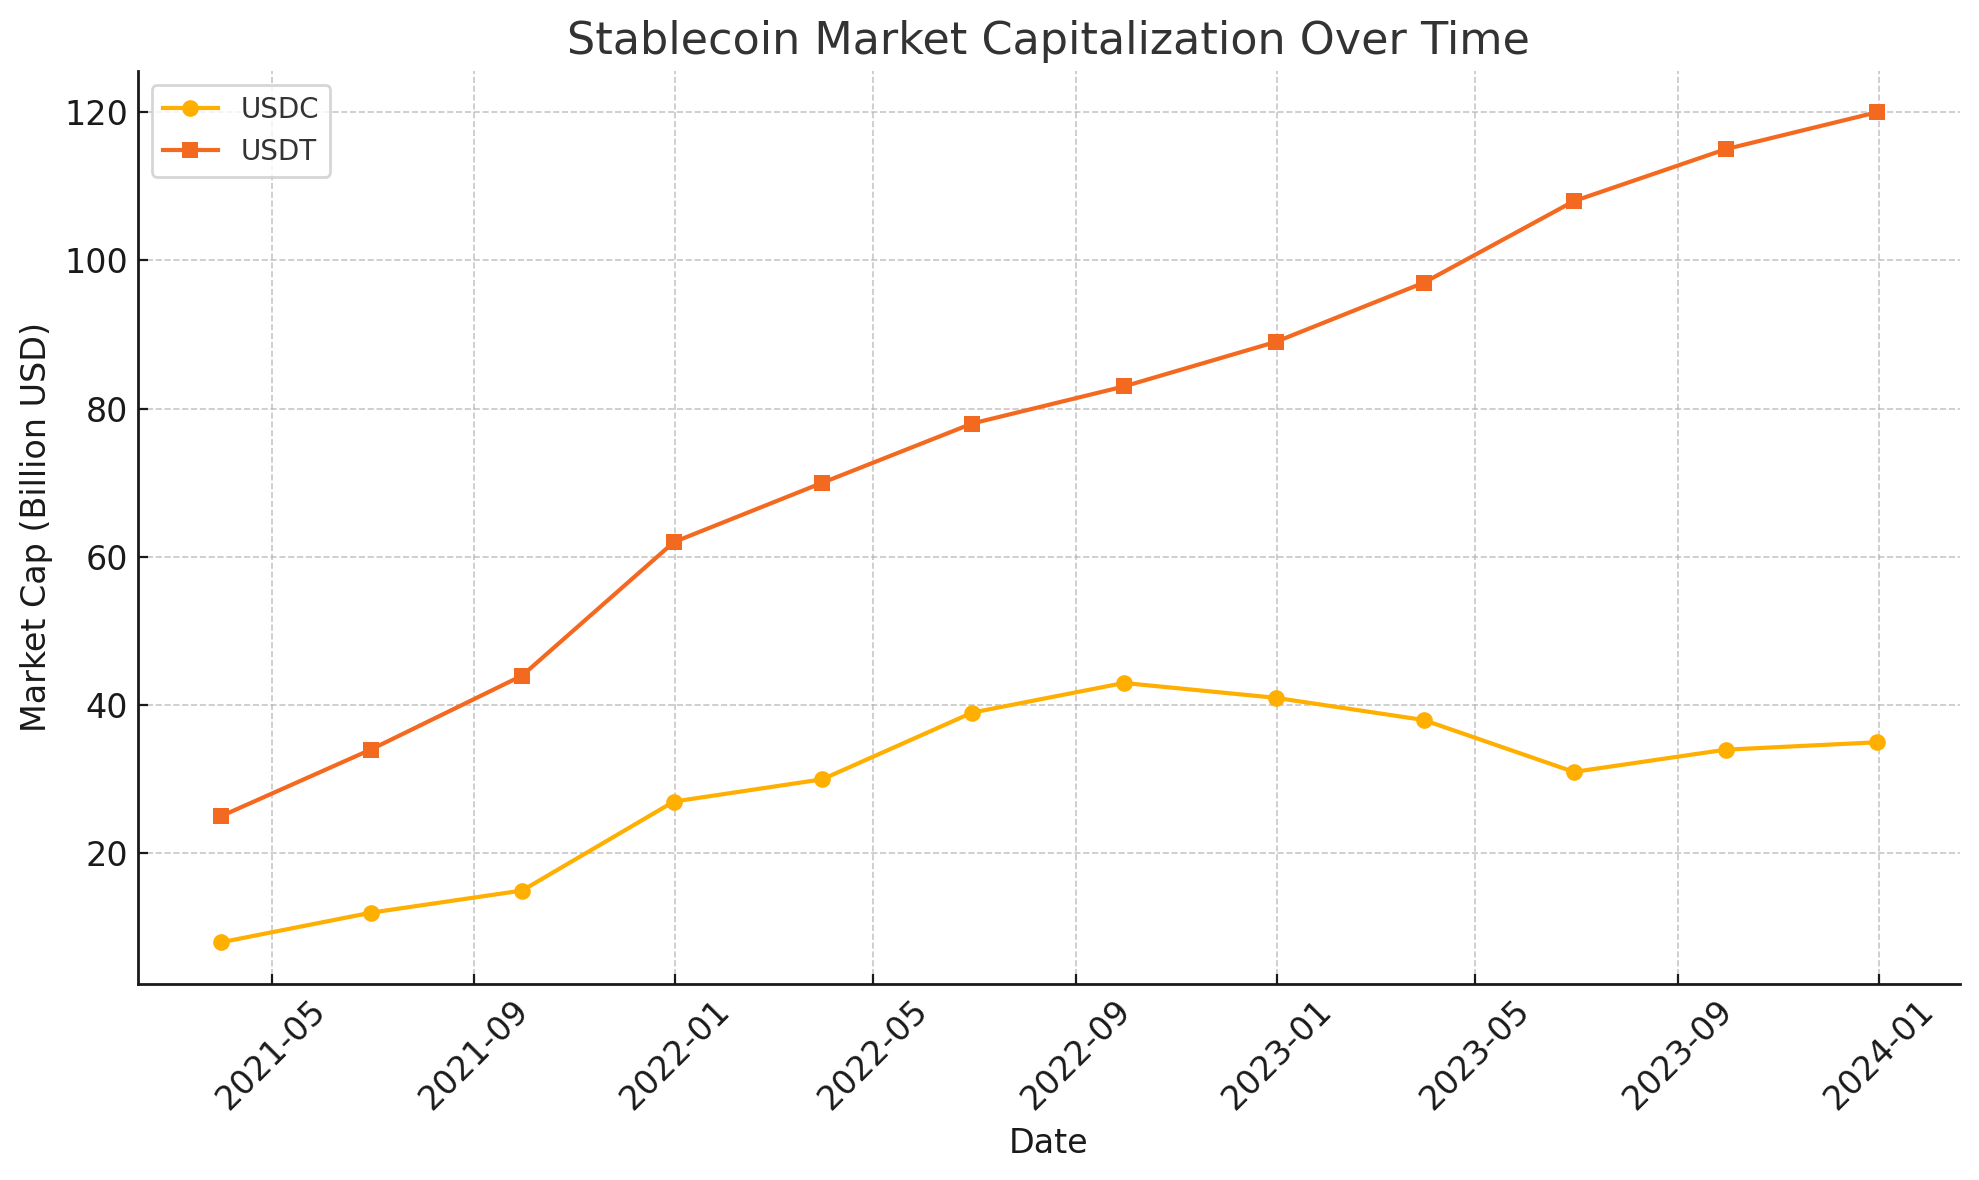
\includegraphics[width=0.8\linewidth]{Figure1.png}\\
\end{frame}

\begin{frame}{Stablecoin Reserve Comparison (2024 Snapshot)}
\footnotesize
\renewcommand{\arraystretch}{1.3}
\begin{tabular}{@{}p{3.6cm}p{3.6cm}p{3.6cm}@{}}
\toprule
\textbf{Metric} & \textbf{USDC (Circle)} & \textbf{USDT (Tether)} \\
\midrule
Market Cap      & \$34.7B                & \$118--163B \\
Liquidity Ratio & $\sim$93\% liquid      & $\sim$81.5\% liquid \\
Main Holdings   & Treasuries, repo       & Treasuries, crypto, gold \\
Audit Frequency & Monthly attestations \& audits & Monthly attestations only \\
Stress Events   & Mar 2023 (SVB exposure) & Oct 2018, 2021, Terra 2022 \\
\bottomrule
\end{tabular}
\vspace{0.5em}

\textit{Source: Circle, Tether transparency reports, IMF Crypto Monitor (2025).}
\end{frame}


\begin{frame}{Launching a Stablecoin}
\small
\begin{itemize}

    \item A private consortium issues a currency fully \textbf{backed by a basket of risk-free securities} denominated in government currency.

    \vspace{0.6em}

    \item The consortium buys and sells the private currency at an arbitrarily chosen exchange rate $\mathcal{E}_t$, 
    investing proceeds $M_t^*\mathcal{E}_t$ in safe bonds.  
    These bonds yield $(1+i_t)M_t^*\mathcal{E}_t$, from which a management fee 
    $\phi_t^f M_t^*\mathcal{E}_t$ is deducted.

    \vspace{0.6em}

    \item To credibly promise repurchases of its currency, the exchange rate must satisfy:
    \begin{align}
        \mathcal{E}_{t+1} 
        &= (1 + i_t - \phi_t^f)\,\mathcal{E}_t.
        \tag{2.50}\label{2.50}
    \end{align}

    \vspace{0.8em}

    \item \textbf{Implications:}
    \begin{itemize}
        \item If $\phi_t^f < i_t$:  
              $\mathcal{E}_t$ \textbf{appreciates}; government money is crowded out.
        \item If $\phi_t^f > i_t$:  
              only government currency is used.
        \item If $\phi_t^f = i_t$:  
              both currencies coexist — the private currency is a \textbf{stablecoin}.
    \end{itemize}

\end{itemize}
\end{frame}

\begin{frame}{Stablecoins: Key Takeaways}
\small
\begin{itemize}

    \item A stablecoin is a \textbf{privately issued synthetic dollar} designed to maintain a near-par exchange rate with government currency ($\mathcal{E}_t \approx 1$).

    \vspace{0.3em}

    \item Credible stability requires \textbf{high-quality backing} (e.g., short-term Treasuries) and a \textbf{redemption commitment} at the chosen exchange rate.

    \vspace{0.3em}

    \item Backing generates a \textbf{carry return} for the issuer. Under the pricing condition
    \[
        \mathcal{E}_{t+1}=(1+i_t-\phi_t^f)\mathcal{E}_t,
    \]
    the management fee $\phi_t^f$ determines whether the private currency appreciates, is stable, or depreciates.

    \vspace{0.3em}

    \item If issuers rebate part of the backing returns to users (low $\phi_t^f$), stablecoins can become a \textbf{high-return medium of exchange} and potentially \textbf{crowd out government money}.

    \vspace{0.3em}

    \item Conversely, maintaining government currency dominance requires keeping inflation low and/or regulating stablecoin backing and payout policies.

\end{itemize}
\end{frame}


% =====================================================
\section{Summary}
% =====================================================


\begin{frame}{Main Takeaways}
\small
\begin{itemize}

    \item A fiduciary-currency system is a historical discontinuity: currency becomes a \textbf{self-referential claim}, yet remains essential for payments.

    \vspace{0.2em}

    \item Controlling monetary aggregates alone cannot uniquely determine the price level — capital backing, taxes, or convertibility must complete the system.
    
\vspace{0.2em}

    \item Seigniorage may also provide a \textbf{real backing} for currency.

    \vspace{0.2em}

    \item Under the Gold Standard, the price level is anchored by the \textbf{value of gold} and by its limited supply.

    \vspace{0.2em}

    \item The \textbf{Friedman rule} prescribes satiating real money balances and achieving deflation at rate $\beta$.

    \vspace{0.2em}

    \item Currency competition shows that a “strong” private currency (or a stablecoin with backing) can \textbf{crowd out government money}, disciplining inflation.

\end{itemize}
\end{frame}


% =====================================================
\section{Bibliography}
% =====================================================

\begin{frame}{References}
\printbibliography
\end{frame}

\end{document}
